\section{Prototype}
\label{sec:implementation:prototype}

This section presents the prototype of the Android Wear application as well as the \emph{binding}, i.e. an addon providing functionality specific to a problem domain, for openHAB developed during the project.

\subsection{Android Wear}
\label{sec:implementation:prototype:android-wear}

\Cref{fig:implementation:prototype:navigation-diagram} shows a navigation diagram of the smart watch application. The letters in the top right corner of the nodes in the diagram references the screenshots shown in \cref{fig:implementation:prototype:screenshots}.

For a list of the supported features in the application, please refer to \cref{sec:implementation:status}.

\begin{figure}[!htb]
    \centering
    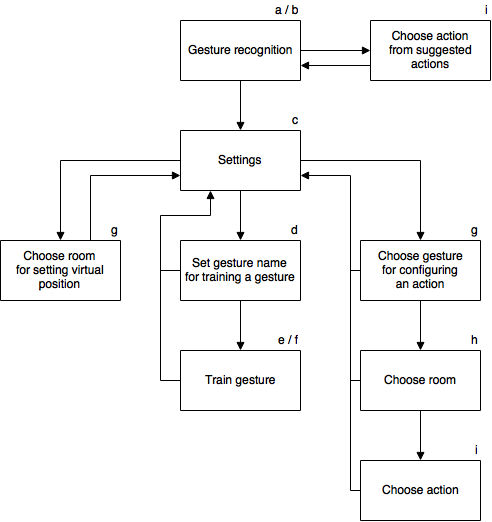
\includegraphics[width=0.7\textwidth]{images/wear-navigation-diagram}
    \caption{Navigation diagram of the application developed for the Android Wear device. Letters in the top right corner of each node refers to the screenshots in figure \cref{fig:implementation:prototype:screenshots}.}
    \label{fig:implementation:prototype:navigation-diagram}
\end{figure}

\begin{figure}[!htb]%
    \centering
    \subbottom[Screen on which the user can start gesture recognition by touching the screen.]{\label{fig:implementation:protoype:screenshots:1}
        \frame{
\includegraphics[width=0.3\textwidth]{images/wear-screenshot-touch-recognize}}
    }
    \subbottom[Screen on which the user can stop gesture recognition by touching the screen. The orange color indicates that recognition has been started.]{\label{fig:implementation:prototype:screenshots:2}
        \frame{
\includegraphics[width=0.3\textwidth]{images/wear-screenshot-recognizing}}
    }
    \subbottom[Settings screen from which the user can set his virtual, train a gesture and configure a new action (create a gesture configuration). When a virtual position is set, the setting can be selected again to unet the virtual position.]{\label{fig:implementation:prototype:screenshots:3}
        \frame{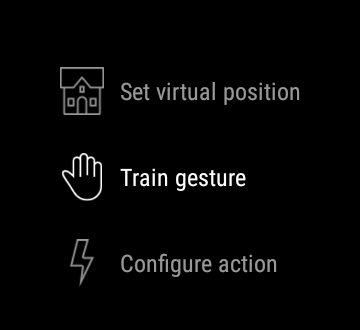
\includegraphics[width=0.3\textwidth]{images/wear-screenshot-settings}}
    }
    \subbottom[Screen shown when the user starts training a gesture. Tapping the ``Gesture name'' button will present the user with a speech recognition interface from which he pronounce the name of the gesture to configure it.]{\label{fig:implementation:protoype:screenshots:4}
        \frame{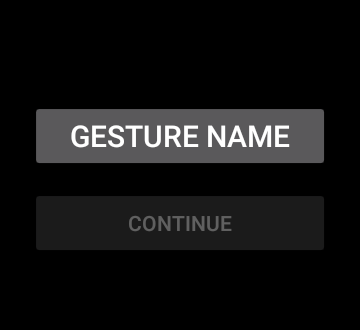
\includegraphics[width=0.3\textwidth]{images/wear-screenshot-name-gesture}}
    }
    \subbottom[Screen shown when training a gesture and the gesture recognizer has not been started. We see that two gesture samples, i.e. gesture templates, have been trained.]{\label{fig:implementation:prototype:screenshots:5}
        \frame{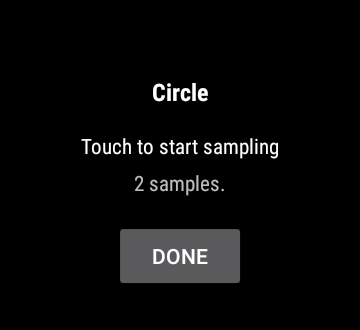
\includegraphics[width=0.3\textwidth]{images/wear-screenshot-touch-train}}
    }
    \subbottom[Screen shown when training a gesture and the gesture recognizer has been started, i.e. the user is performing a gesture.]{\label{fig:implementation:prototype:screenshots:6}
        \frame{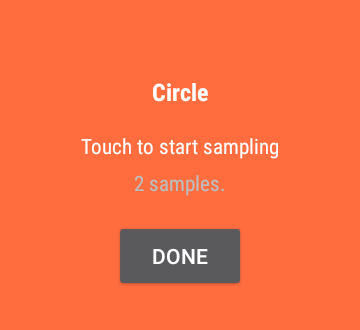
\includegraphics[width=0.3\textwidth]{images/wear-screenshot-training}}
    }
    \subbottom[Gesture picker showing the gestures the user has trained. The gesture picker is used when creating a gesture configuration.]{\label{fig:implementation:protoype:screenshots:7}
        \frame{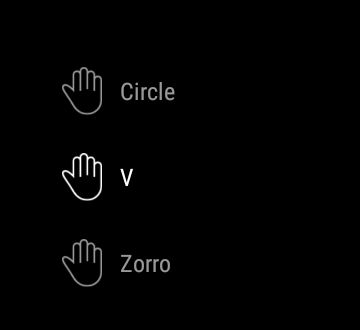
\includegraphics[width=0.3\textwidth]{images/wear-screenshot-gestures}}
    }
    \subbottom[Room picker shown when the user creates a gesture configuration. The picker is also shown when setting a virtual position.]{\label{fig:implementation:prototype:screenshots:8}
        \frame{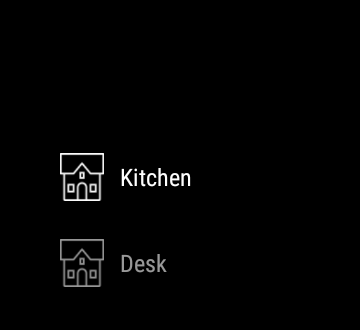
\includegraphics[width=0.3\textwidth]{images/wear-screenshot-rooms}}
    }
    \subbottom[Action picker shown when creating a gesture configuration. A similar picker is shown when the context engine suggests multiple actions.]{\label{fig:implementation:prototype:screenshots:9}
        \frame{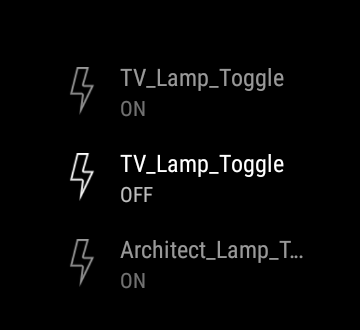
\includegraphics[width=0.3\textwidth]{images/wear-screenshot-actions}}
    }
    \caption{Screenshots of the prototype developed for the Android Wear smart watch.}
    \label{fig:implementation:prototype:screenshots}
\end{figure}

\subsection{openHAB}
\label{sec:implementation:prototype:openhab}

We developed a \emph{binding} for openHAB. A \emph{binding} is an addon for openHAB which relates to a specific problem domain. For example, there is a binding for communcating with Philips Hue lights and a binding for controlling a Sonos media centre. We have created a binding for configuring the rooms and beacons in a users home.

We chose to place the configuration of the rooms and beacons in openHAB, as this is a one time configuration which can be shared amongst the users in a home where as the creation of gesture configurations is place on the watch as this can be independent for each inhabitant of a home.

The rooms and beacons are synchronized to the smart watch when the application is loaded. The watch use the models when positioning the user.

A room has a name and when it is created, openHAB assigns it a UID. When creating a beacon, the user must enter the UID assigned by openHAB in order to specify which room the beacon is placed in. Furthermore the user should enter the Eddystone namespace and instance, both described in \cref{sec:design:ble-positioning}. This identifies the specific beacon. When the smart watch registers a beacon, it can determine which room the user is in by the beacons reference to a room.

% \begin{figure}[!htb]%
%     \centering
%     \subbottom[Screen on which to choose the binding to configure.]{\label{fig:implementation:protoype:openhab:bindings}
%         \frame{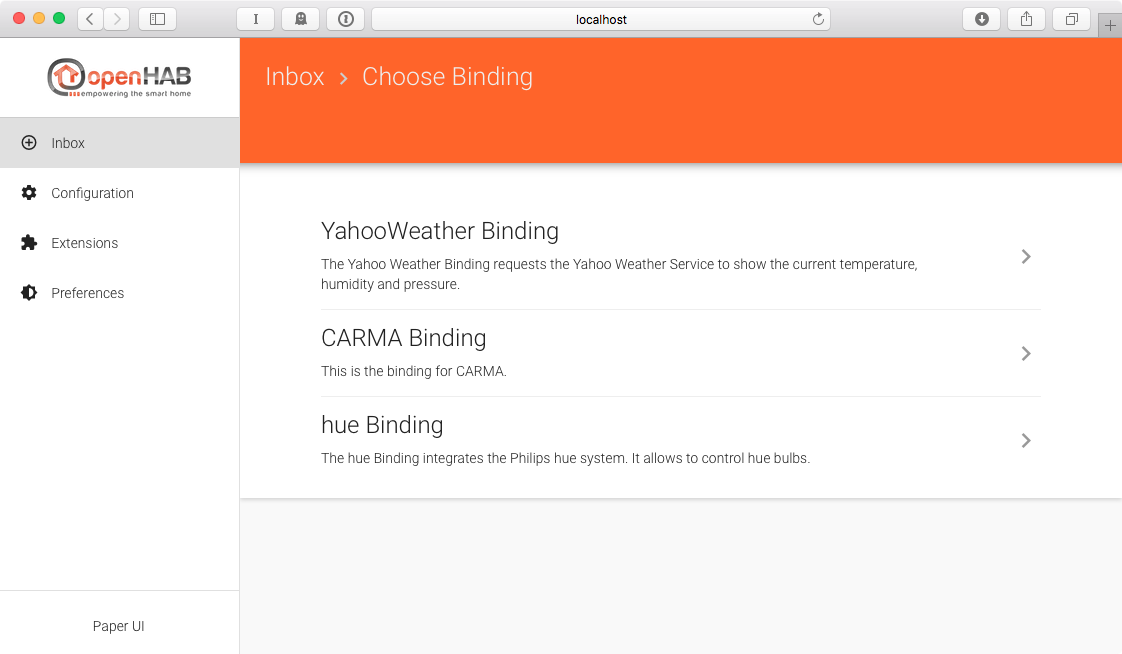
\includegraphics[width=0.5\textwidth]{images/openhab-addon-bindings}}
%     }
%     \subbottom[Screen on which the \emph{thing} to create is chosen. In openHAB physical devices are referred to as \emph{things}.]{\label{fig:implementation:prototype:openhab:things}
%         \frame{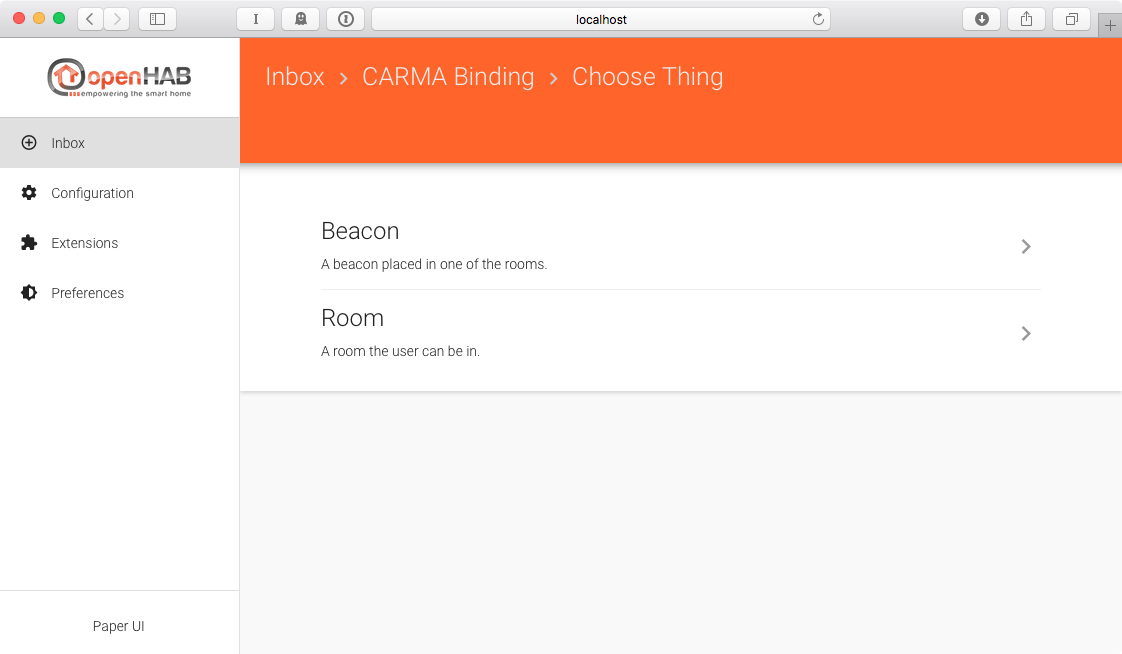
\includegraphics[width=0.45\textwidth]{images/openhab-addon-things}}
%     }
%     \subbottom[Screen on which a new room can be created. The room should have a name, e.g. ``Kitchen'' or ``Living room''.]{\label{fig:implementation:protoype:openhab:room}
%         \frame{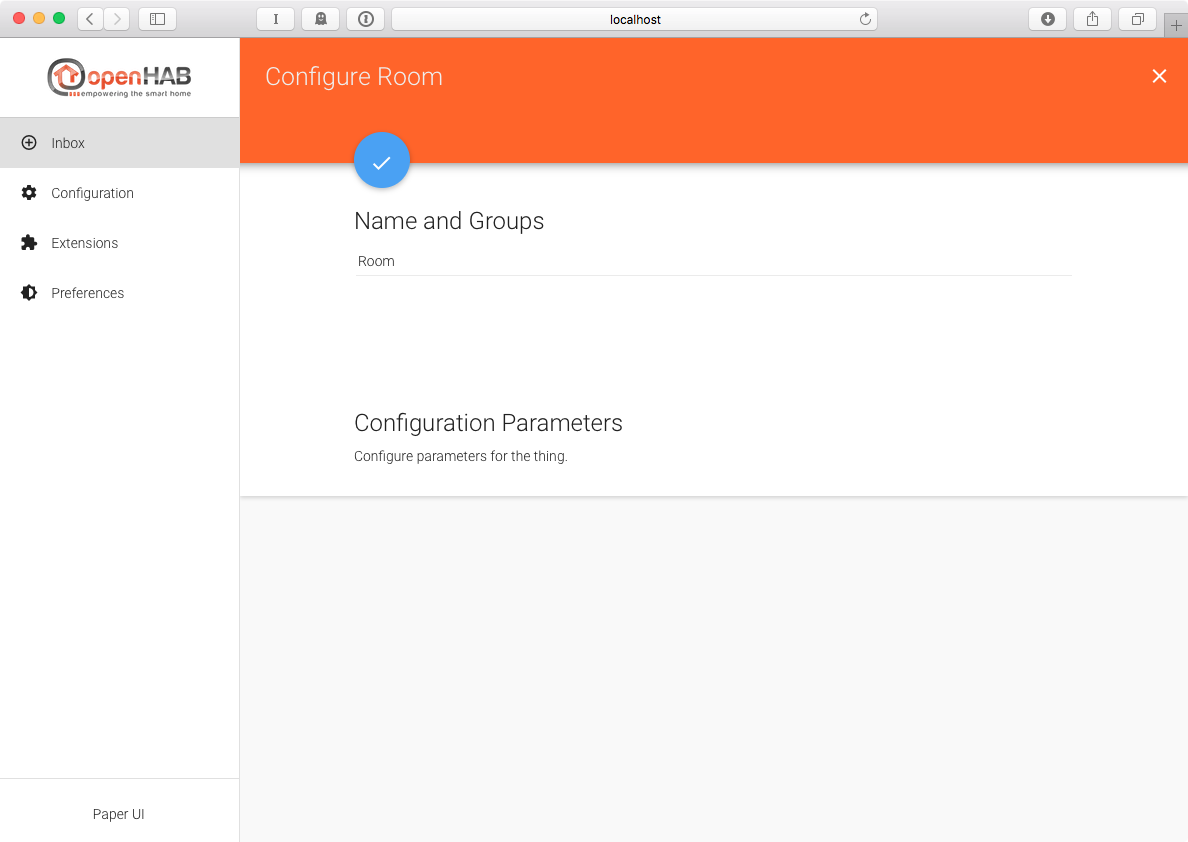
\includegraphics[width=0.45\textwidth]{images/openhab-addon-room}}
%     }
%     \subbottom[Screen on which a new beacon can be created. The UID of the room the beacon is placed in must be specified. UIDs are created by openHAB when a new room is created. The namespace and instance of the Eddystone beacon must also be specified. ]{\label{fig:implementation:prototype:openhab:beacon}
%         \frame{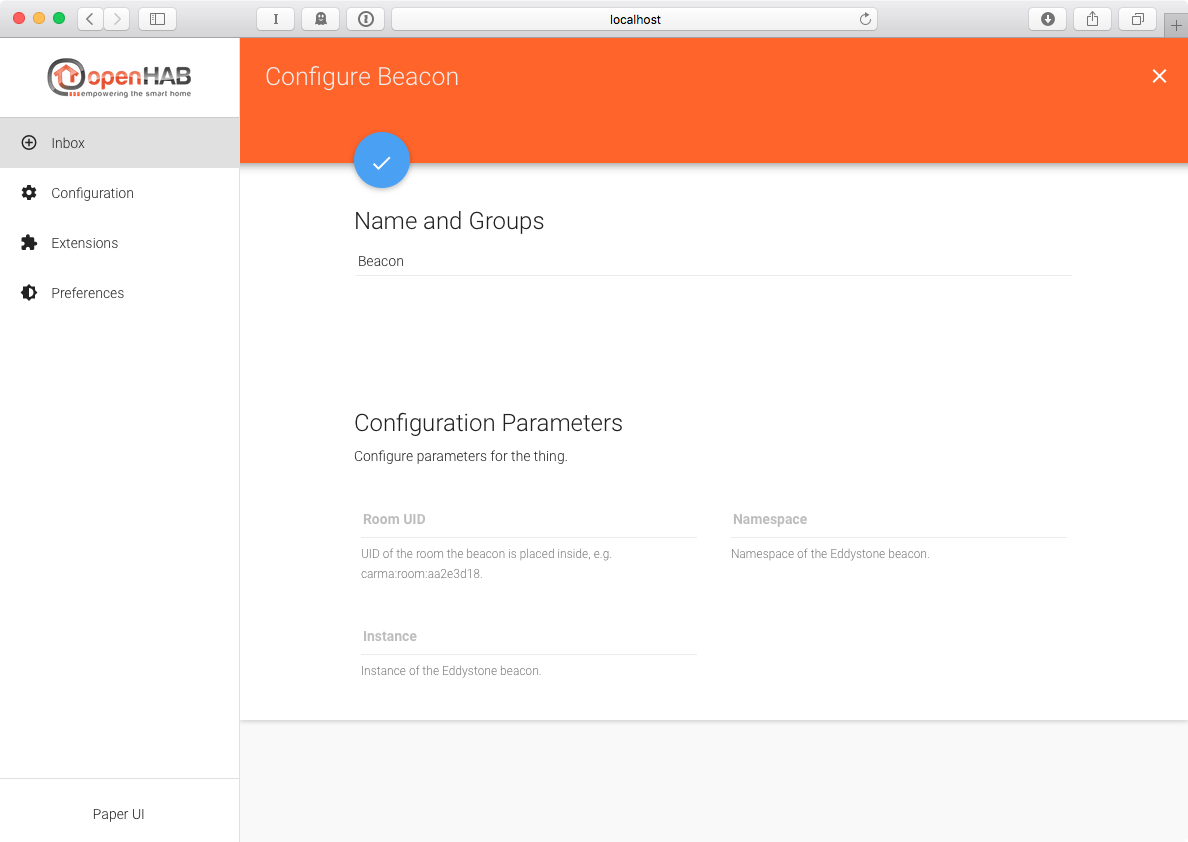
\includegraphics[width=0.45\textwidth]{images/openhab-addon-beacon}}
%     }
%     \subbottom[Screen showing the list of all configured things in openHAB. The screenshot shows two rooms and two beacons configured as well as some Philips Hue light bulbs.]{\label{fig:implementation:prototype:openhab:list}
%         \frame{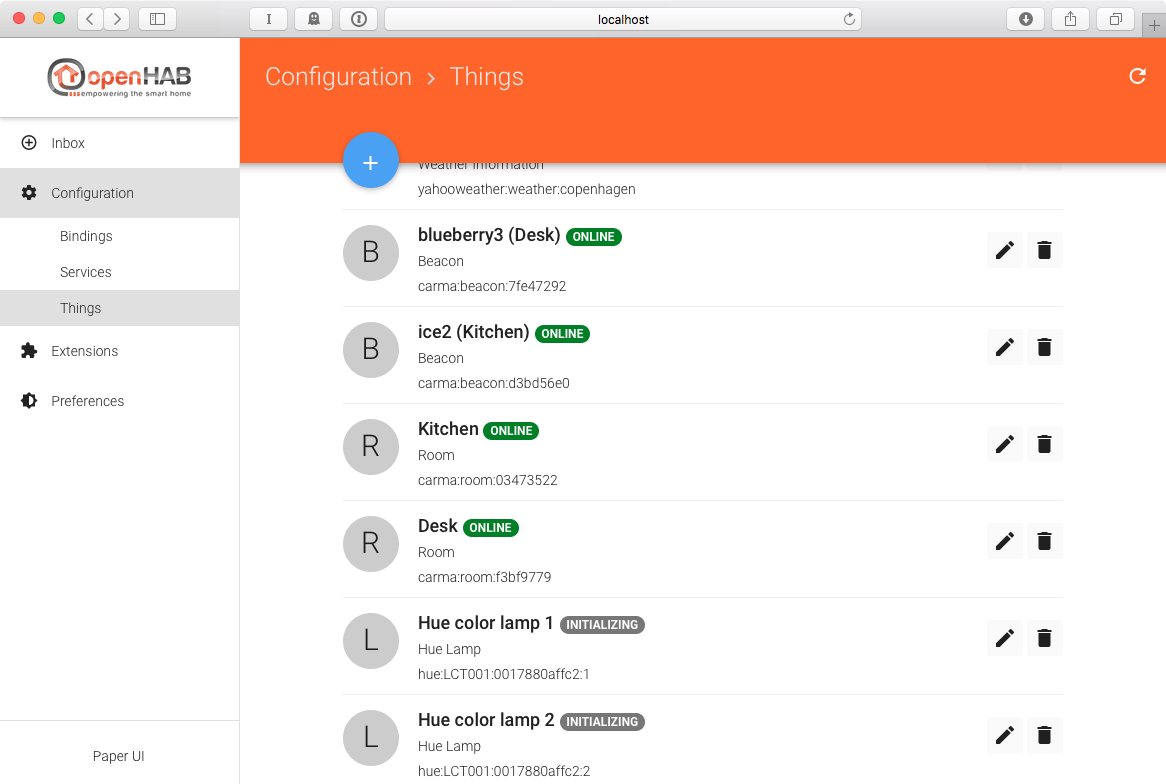
\includegraphics[width=0.45\textwidth]{images/openhab-addon-list}}
%     }
%     \caption{Screenshots of the binding developed for openHAB.}
%     \label{fig:implementation:prototype:openhab:screenshots}
% \end{figure}

%%% Local Variables:
%%% mode: latex
%%% TeX-master: "../../master"
%%% End:
